\section{Overview}\label{sec:overview}

\begin{figure}
  \centering
  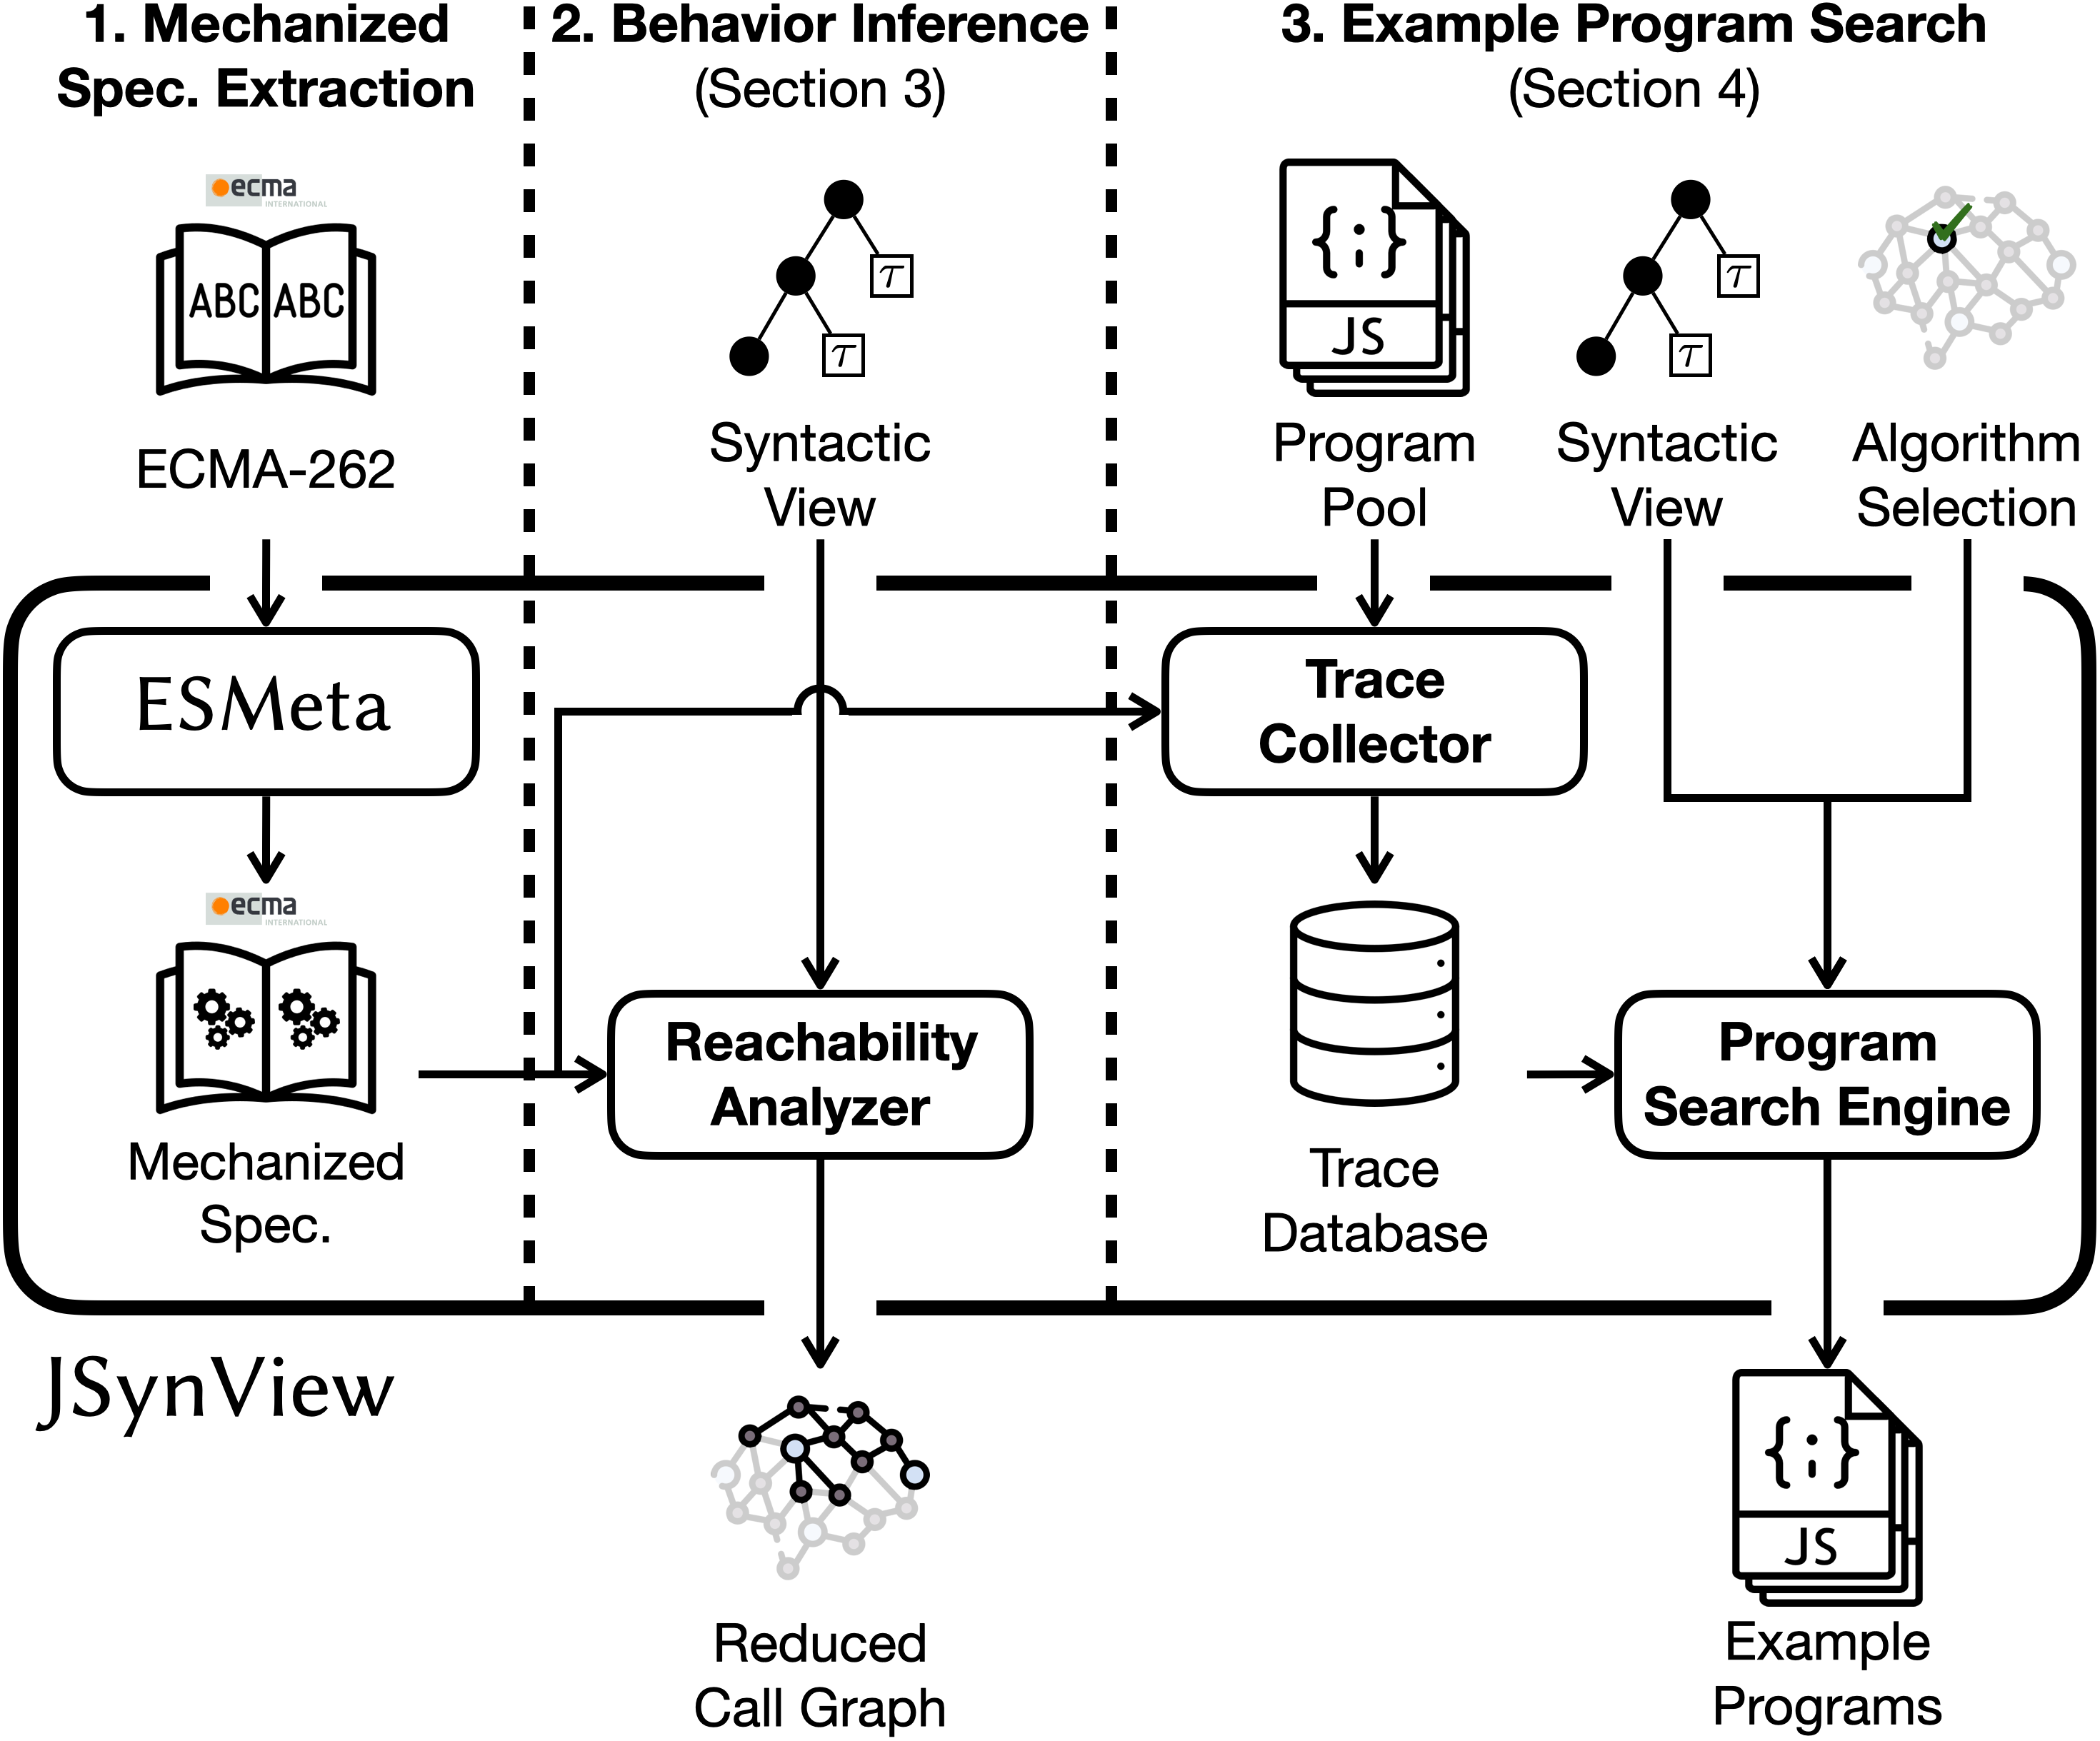
\includegraphics[width=\columnwidth]{img/overall.png}
  \caption{Overall structure of $\tool$}
  \vspace*{-1em}
  \label{fig:overall}.
\end{figure}

\begin{figure}
  \centering
  \begin{subfigure}[t]{\columnwidth}
    \centering
    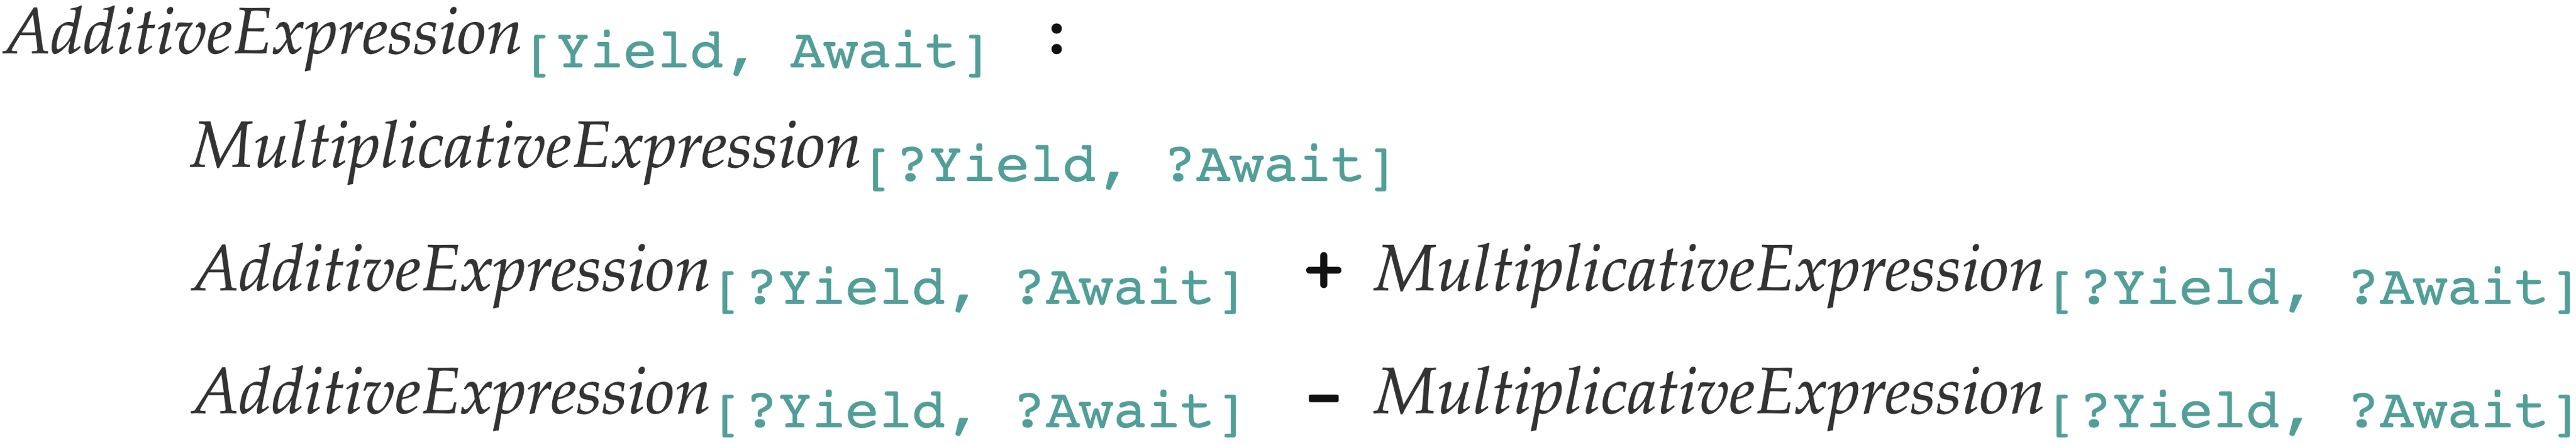
\includegraphics[width=\columnwidth]{img/add-eval-bnf.png}
    \caption{The \essyn{AdditiveExpression} production for syntax}
  \end{subfigure}
  \vspace*{.5em}
  \begin{subfigure}[t]{\columnwidth}
    \centering
    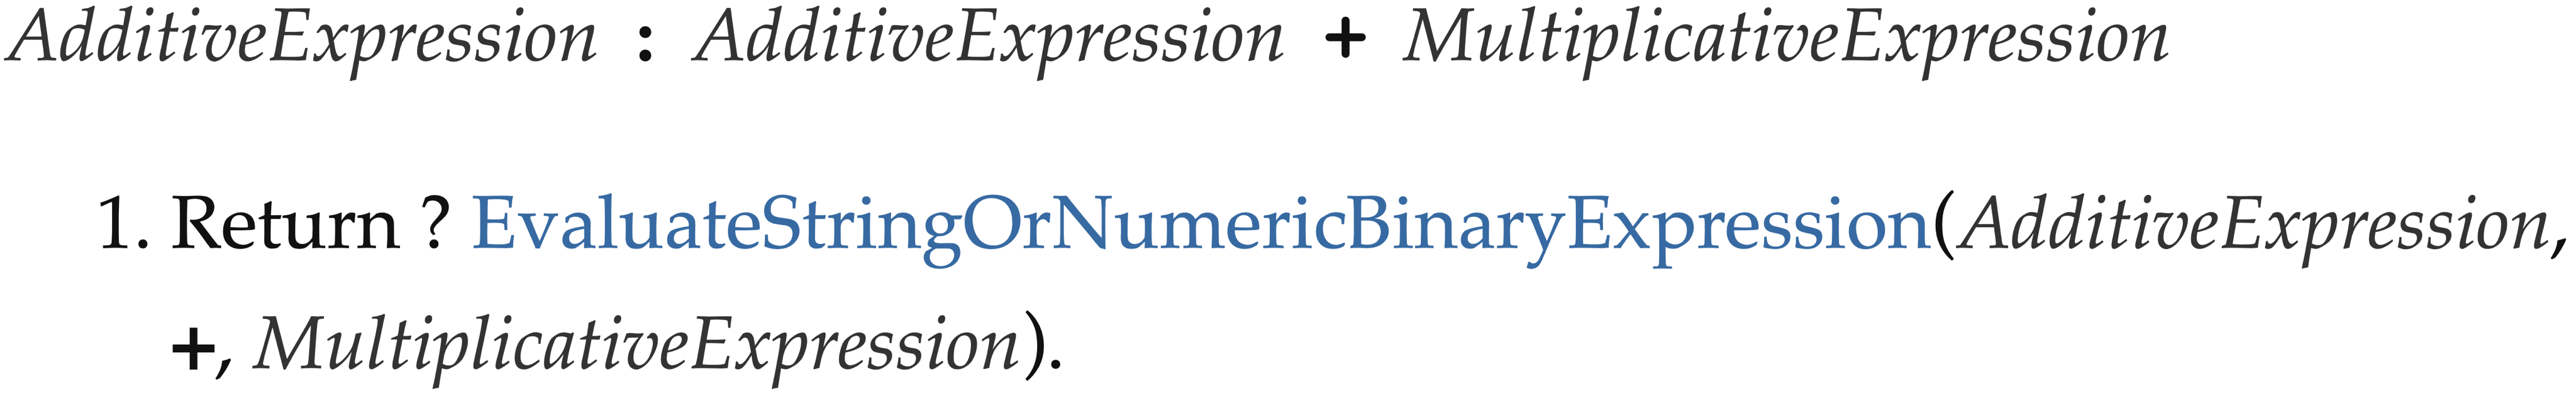
\includegraphics[width=\columnwidth]{img/add-eval-algo.png}
    \caption{The \esalg{Evaluation} algorithm of for semantics}
  \end{subfigure}
  \vspace*{-.5em}
  \caption{The syntax and semantics of the addition expression in the latest
  ECMA-262 (ES13, 2022)}
  \vspace*{-1.5em}
  \label{fig:add-eval}
\end{figure}

\begin{figure*}
  \centering
  \begin{minipage}[b]{\columnwidth}
    \begin{subfigure}[t]{\columnwidth}
      \centering
      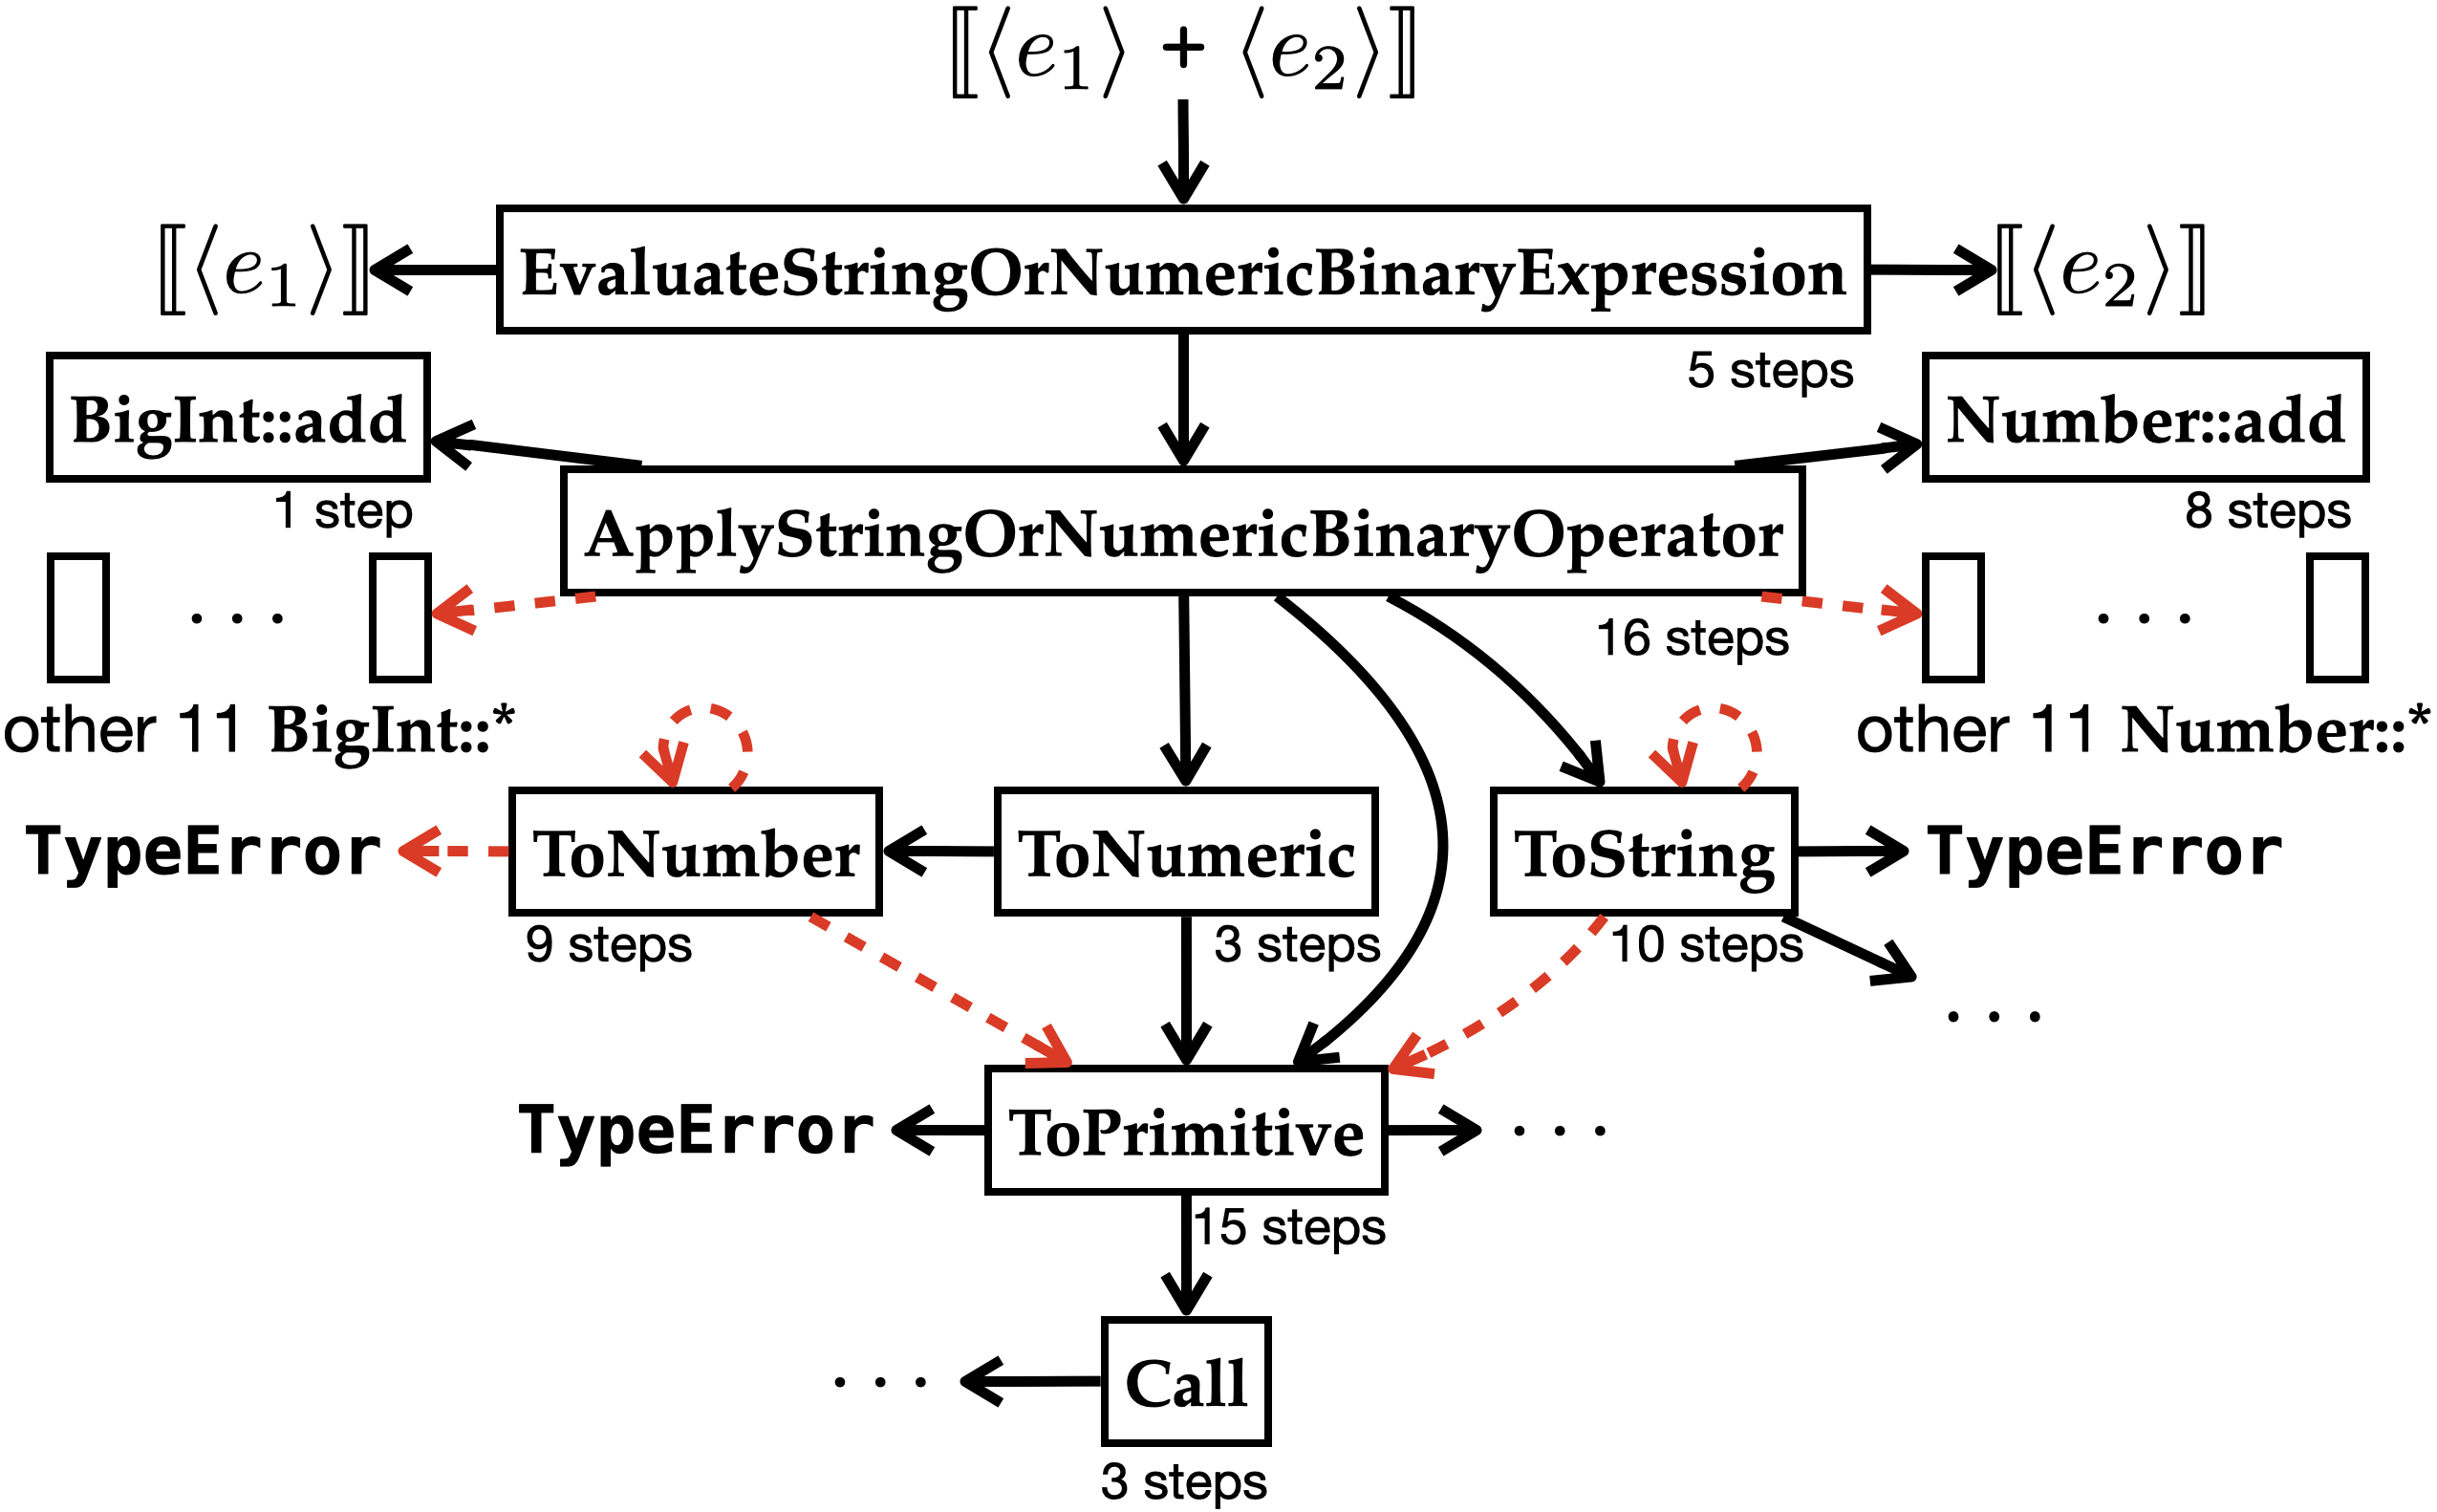
\includegraphics[width=\textwidth]{img/add-basic.png}
      \caption{Reduced call graph with $\svhole{\expr_1} \; \code{+} \;
      \svhole{\expr_2}$}
    \end{subfigure}
  \end{minipage}
  \begin{minipage}[b]{\columnwidth}
    \begin{subfigure}[t]{\columnwidth}
      \centering
      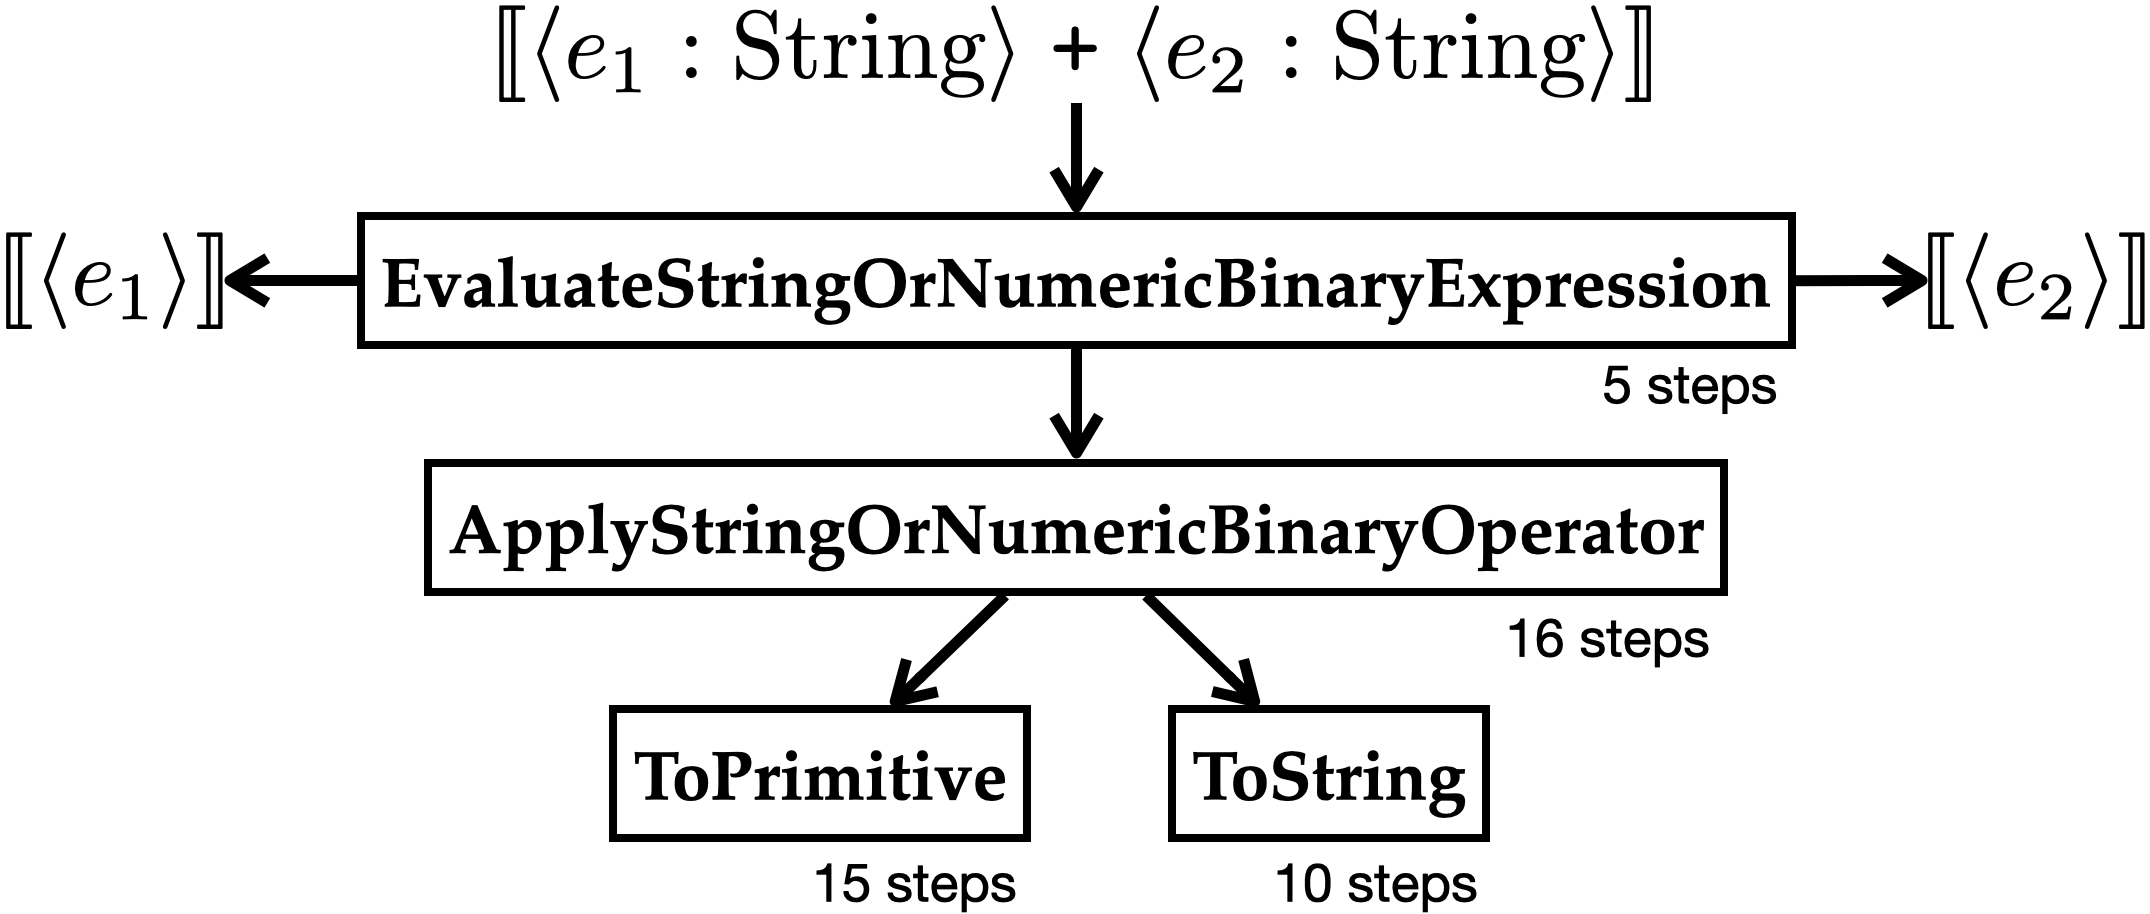
\includegraphics[width=.8\textwidth]{img/add-str.png}
      \caption{Reduced call graph with $\svhole{\expr_1: \text{String}} \;
      \code{+} \; \svhole{\expr_2: \text{String}}$}
    \end{subfigure}
    \begin{subfigure}[t]{\columnwidth}
      \centering
      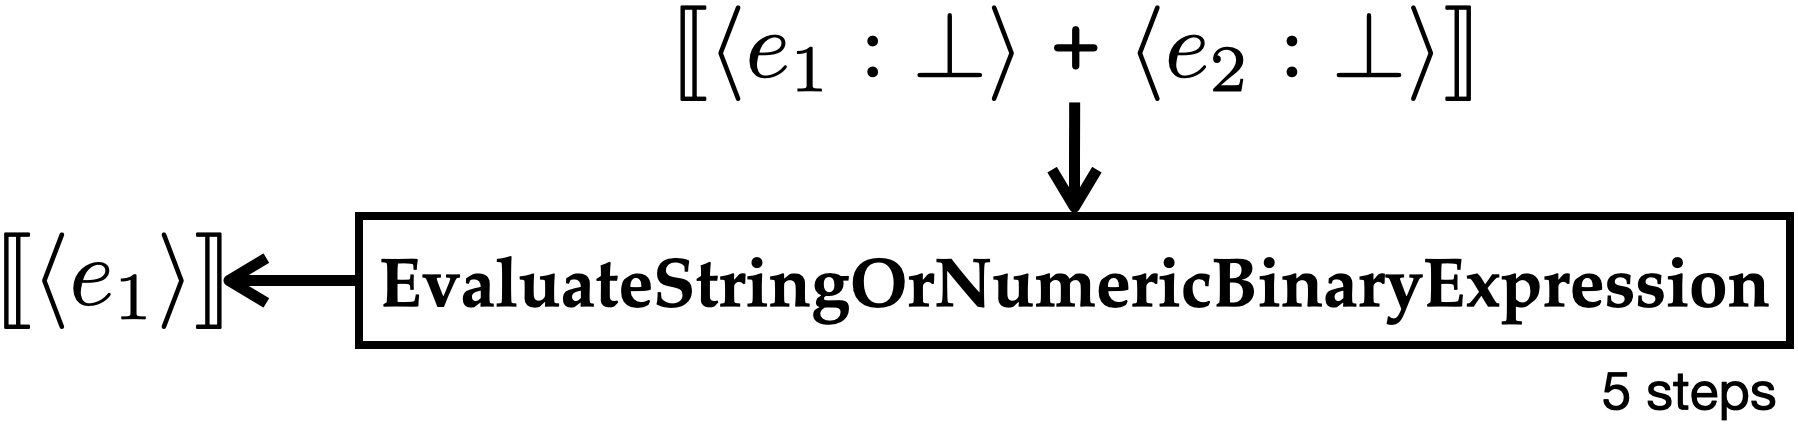
\includegraphics[width=.7\textwidth]{img/add-exc.png}
      \caption{Reduced call graph with $\svhole{\expr_1: \bot} \; \code{+} \;
      \svhole{\expr_2: \bot}$}
    \end{subfigure}
  \end{minipage}
  \vspace*{-.5em}
  \caption{Reduced call graphs of ECMA-262 with three different syntactic views}
  \vspace*{-1.5em}
  \label{fig:add-graph}.
\end{figure*}

This section explains the overall structure of $\tool$ depicted in
Figure~\ref{fig:overall} with simple examples.  It consists of three modules: 1)
\textit{mechanized specification extraction}, 2) \textit{behavior inference} and
3) \textit{example program search}.


\subsection{Mechanized Specification Extraction}\label{sec:extract-spec}

$\tool$ first extracts a \textit{mechanized specification} from ECMA-262, the
standard JavaScript language specification written in English.

ECMA-262 describes the syntax using a variant of the extended Backus–Naur form
and the semantics as abstract algorithms.  Each algorithm describes the language
semantic in a procedural way with structured steps.  For example,
Figure~\ref{fig:add-eval} (a) shows the syntactic production of
\essyn{AdditiveExpression} in the latest ECMA-262 (ES13, 2022)~\cite{es13}.
Figure~\ref{fig:add-eval} (b) shows the \esalg{Evaluation} algorithm of its
second alternative that describes the semantics of the addition
expression.\footnote{\url{https://262.ecma-international.org/13.0/\#sec-addition-operator-plus}}
It consists of a single step that invokes another algorithm,
\esalg{EvaluateStringOrNumericBinaryExpression}; the first and third arguments
are the left and right subtrees of the abstract syntax tree (AST) for a given
addition expression, and the second one is a text \code{+} to represent the
addition operation.  The \esalg{EvaluateStringOrNumericBinaryExpression} is a
generic algorithm for string or numeric binary operations (e.g., \code{-},
\code{*}, \code{<}, etc.).

However, it is difficult to handle it in an automatic or mechanical way since it
is written in English.  Thus, we utilize another tool $\esmeta$~\cite{jiset,
esmeta}, which extracts a mechanized specification from any given version of
ECMA-262.  It automatically converts algorithms steps to the corresponding
instructions of $\ires$, an intermediate representation for ECMAScript.  In
other word, the mechanized specification extracted via $\esmeta$ is an $\ires$
program consisting of functions corresponding to abstract algorithms in the
language specification.


\subsection{Behavior Inference}\label{sec:reduce-spec}

\name{Reachability Analyzer} takes a mechanized specification and performs its
reachability analysis to automatically reduce the call graph of ECMA-262 with a
given \textit{syntactic view} to soundly infer \textit{possible behaviors}.  A
\textit{syntactic view} is an extension of a JavaScript abstract syntax tree
(AST) consisting of both concrete and abstract nodes with type bounds.
Users can freely construct syntactic views depending on which combination of
language features they want to understand; concrete nodes denote the parts they
want to understand, and abstract ones denote the parts they do not.  Then, the
analyzer takes such a syntactic view as the target language features and
performs reachability analysis based on abstract interpreter
framework~\cite{ai1977, ai1992}.  Finally, it builds the reduced call graph of
ECMA-262 using the analysis result, and we can soundly infers \textit{possible
behaviors} of language features using the reduced call graph.


\subsubsection{Examples with Simple Syntactic Views}

Assume that we want to understand the detailed semantics of JavaScript addition
operation by referring to ES13.  Then, we can utilize a syntactic view
$\svhole{\expr_1} \; \code{+} \; \svhole{\expr_2}$ where $\svhole{\expr_1}$ and
$\svhole{\expr_2}$ denote abstract nodes for \essyn{AdditiveExpression} and
\essyn{MultiplicativeExpression}, respectively.  With this syntactic view, the
analyzer starts the analysis from the \esalg{Evaluation} algorithm shown in
Figure~\ref{fig:add-eval} (b) and builds a call graph depicted in
Figure~\ref{fig:add-graph} (a) consisting of \inred{109} algorithms.  In this
graph, a node denotes 1) an abstract algorithm (box), 2) evaluation of syntactic
view ($\sem{-}$), or 3) an exception (bold without box), and an arrow denotes a
call edge.  Because the analyzer considers the context of evaluating the
addition operation, it removes invalid call edges (red dotted arrows) in the
call graph.  For example, \esalg{ApplyStringOrNumericBinaryOperator} can invoke
only two different numeric methods \esalg{BigInt::add} and \esalg{Number::add}
during the evaluation of the addition operation, and other 22 numeric methods
(e.g., \esalg{Number::divide}) are removed.  In this call graph, specific
algorithms represent possible behaviors of the addition operation.  For
instance, the \esalg{Call} algorithm is used to invoke the \eswrd{[[Call]]}
internal method of a JavaScript function object.  It means that a JavaScript
function might be invoked during the evaluation of the addition operation.
Besides, the addition operation might throw a \esval{TypeError} exception
because it is reachable from the \esalg{Evaluation} algorithm.


\subsubsection{Examples with Advanced Syntactic Views}

Beyond basic syntactic restriction, we can give a more restriction to a
syntactic view with 1) type bounds or 2) combination with other language
features.

For instance, assume that we want to understand the addition between string
values.  Then, we represent such cases using the syntactic view
$\svhole{\expr_1: \text{String}} \; \code{+} \; \svhole{\expr_2: \text{String}}$
with type bounds.  Figure~\ref{fig:add-graph} (b) depicts the reduced call graph
with this syntactic view, and gives more information of the addition operator.
First, the addition between string values never throw exceptions because there
is no reachable exceptions in this call graph.  Second, the string addition
never invoke other JavaScript functions because the \esalg{Call} algorithm is no
longer reachable.  As depicted in Figure~\ref{fig:add-graph} (c), we can even
restrict the expected results of the abstract nodes using exceptions:
$\svhole{\expr_1: \bot} \; \code{+} \; \svhole{\expr_2: \bot}$, where $\bot$
denotes an exception.  In this case, we grasp the information that only the left
operand is evaluated when both operands throw exceptions.

Besides, we can combine different language features in syntactic views.  For
example, a syntactic view $\svhole{\expr_1} \; \code{+} \; \svhole{\expr_2} \;
\code{||} \; \svhole{\expr_3}$ represents the combination of addition and
logical OR operations.


\subsection{Example Program Search}\label{sec:reduce-spec}

$\tool$ also provides \textit{example programs} that trigger possible behaviors
by searching for them in a given JavaScript program pool.

Consider a program pool consists of thousands of JavaScript programs with the
following two programs:
\begin{center}
  \begin{tabular}{c}
    \begin{lstlisting}[style=JS]
...      1 + {valueOf: ()=>1}      1n + 1      ...
    \end{lstlisting}
  \end{tabular}
\end{center}
As depicted in Figure~\ref{fig:add-graph} (a), the reduced call graph for the
addition operation contains the \esalg{Call} algorithm and the \esval{TypeError}
exception.  It means that addition operation might implicitly invoke a function
and throw a \esval{TypeError} exception, respectively.  However, it is
burdensome to manually find example programs that have such behaviors in the
program pool because it contains thousands of JavaScript programs.

Fortunately, $\tool$ can save the time to search for such example programs.
\name{Trace Collector} first executes all JavaScript programs in the program
pool using the mechanized specification extracted from ECMA-262.  Then, using
their execution traces, it records the relations among programs, AST nodes, and
algorithms in \name{Trace Database}.  Then, if a user selects an algorithm as
the target behavior with a syntactic view, \name{Program Search Engine} utilizes
the database to quickly search for example programs in the pool that touches the
selected algorithm in the semantics of the given syntactic view.

For example, assume that we want to search the example programs containing an
addition operation that implicitly invokes a function.  Then, it is enough to
select the \esalg{Call} algorithm with the syntactic view $\svhole{\expr_1} \;
\code{+} \; \svhole{\expr_2}$, and the search engine returns the first program:
\code{1 + \{valueOf: ()=>1\}}.  On the other hand, if we want to find
example programs that throw a \esval{TypeError} exception in addition
operation, it is enough to select the exception with the same syntactic view.
Then, our tool returns the second program: \code{1n + 1}.

In the remainder of this paper, we explain the details of how to infer possible
behaviors with a given syntactic view (Section~\ref{sec:infer}) and how to
search for example programs that trigger such behaviors in the program pool
(Section~\ref{sec:search}.  After we explain the implementation details of
$\tool$ (Section~\ref{sec:impl}) and evaluate it (Section~\ref{sec:eval}, we
discuss related work (Section~\ref{sec:related}) and conclude
(Section~\ref{sec:conclusion}).
